\section{Evaluation}
\label{evaluation}
\label{sec:quantum_eval}


In this section, first, we show the limitation of our baseline method, i.e., a single-level POVM-based method named \povmone.
Then we evaluate the effectiveness of \povm and \povmpro and show that their performance is superior to \povmone. 

\begin{figure}[t]
    \centering
    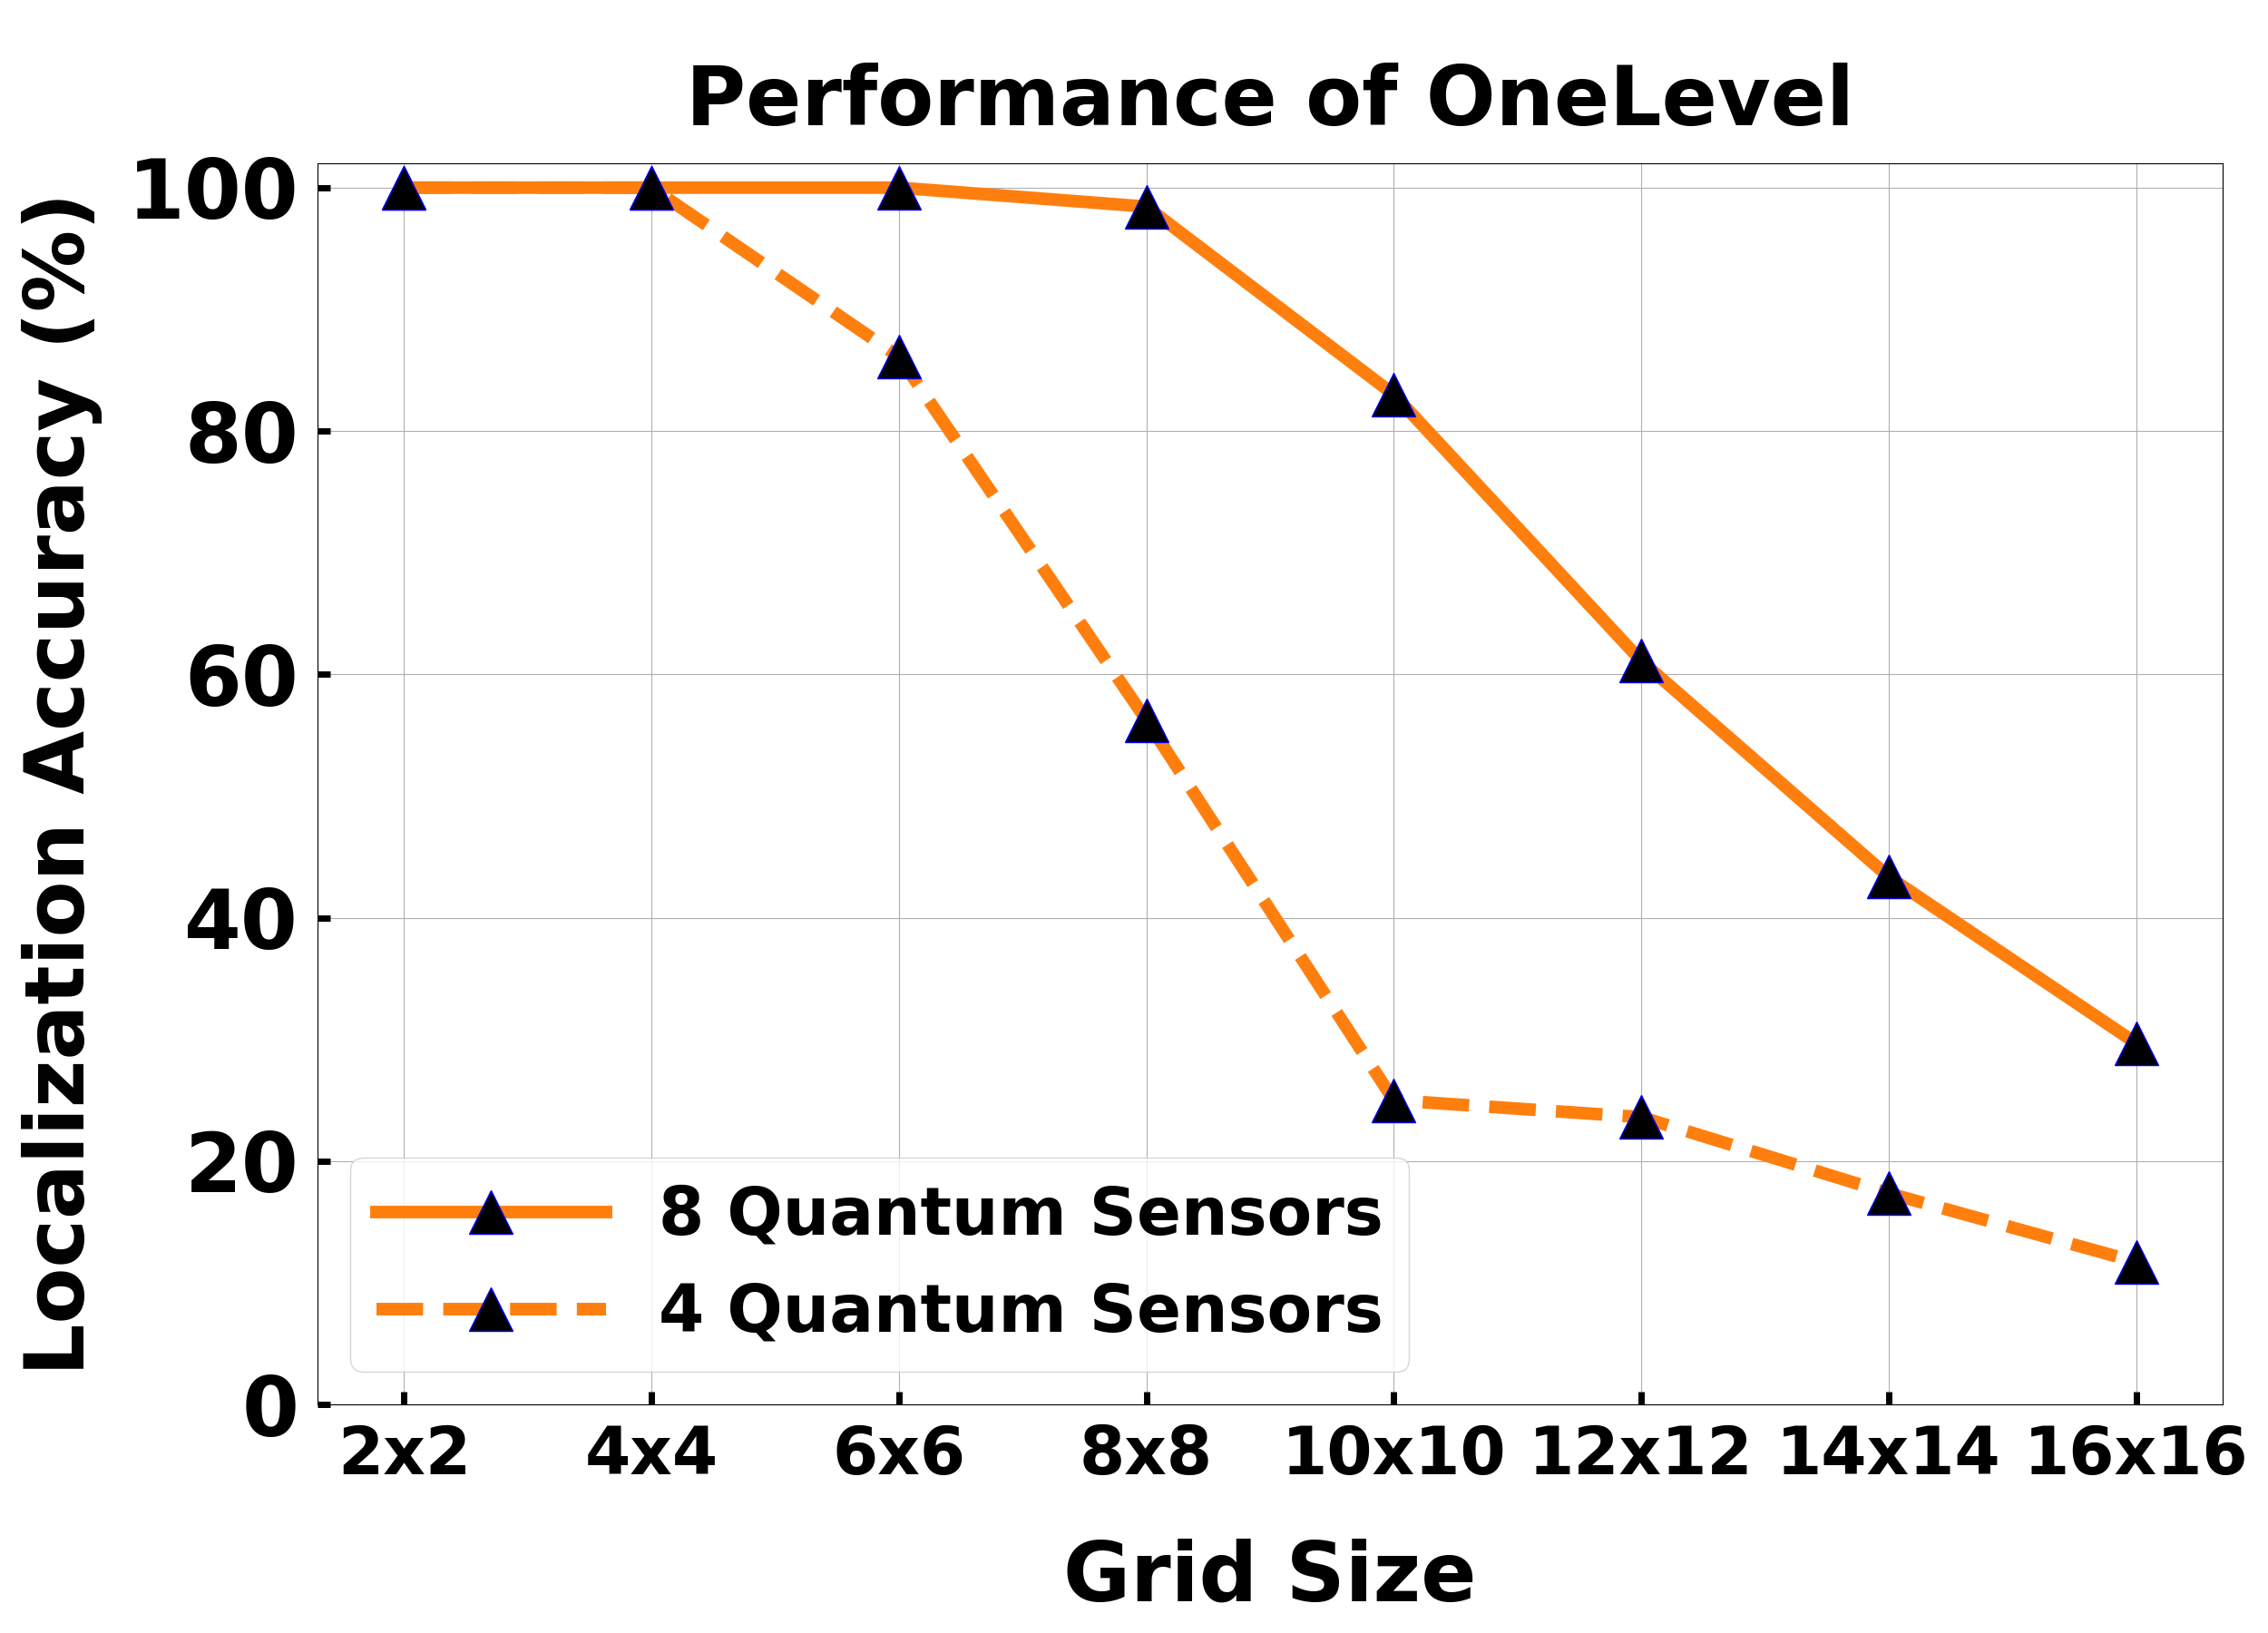
\includegraphics[width=0.75\textwidth]{chapters/icc/figures/onelevel-varygrid.png}
    % \vspace{-0.1in}
    \caption{The performance of \povmone against varying grid size.}
    % \vspace{-0.1in}
    \label{fig:povmloc-onelevel}
\end{figure}

\para{Performance Metrics.} We use the following two metrics to evaluate the localization methods.
\begin{enumerate}
    \item Localization accuracy ($\lacc$)
    \item Localization error ($\lerr$)
\end{enumerate}
$\lacc$ is used for the discrete location setting, where we confine the location of the transmitters during both the training and localization phases to the center of the cells.
$\lerr$ is used for the general continuous location setting, where the transmitters during the localization phase can be anywhere (the transmitters during the training phase are still at the cell center).
Therefore, $\lacc$ is a percentage similar to the classification accuracy, and $\lerr$ is the distance between the ground truth location and the method's output location measured in meters.

\para{Experiment Settings.}
We perform experiments in different grid sizes, while the area of a cell represents stays at $10m \times 10m$.
Our wireless propagation model is the log-distance model in Equation~\ref{equ:propagation}.
Specifically, the reference power $P_0=-10 dBm$, and path-loss exponent $\beta=3.5$.
For the zero-mean normal distribution shadowing effect, the default standard deviation is $1$.
The shadowing effect is considered the source of noise in our evaluation.
In the training phase, the POVM $\{E_i \}$ is computed with data that doesn't contain noise.
In the localization phase, each testing sample (a quantum state reported from quantum sensors) contains noise.
For the location of sensors, we assume the sensors are uniformly spread out to cover the whole area better.


\para{The limitation of \povmone.}
Fig.~\ref{fig:povmloc-onelevel} shows that the localization accuracy of \povmone decreases significantly when the grid size increases.
A larger grid size leads to a larger number of quantum states being discriminated.
This leads to a larger overlap between the quantum states, making the quantum states harder to discriminate.
Fig.~\ref{fig:povmloc-onelevel} also shows that by using 8 quantum sensors, the localization accuracy is higher compared with 4 quantum sensors.
This is because more quantum sensors cover the area better so that the quantum state is able to encode more information about the environment.
More information is encoded in a larger Hilbert space, so the overlap between the quantum states becomes smaller, making the quantum states easier to discriminate.
But the high accuracy brought by a higher number of sensors comes at a cost of higher RAM and runtime, see Table~\ref{tab:runtime-onelevel}.
\povmone's limitation is exactly the challenges mentioned in Section~\ref{sec:our}.




\begin{figure}[t]
    \centering
    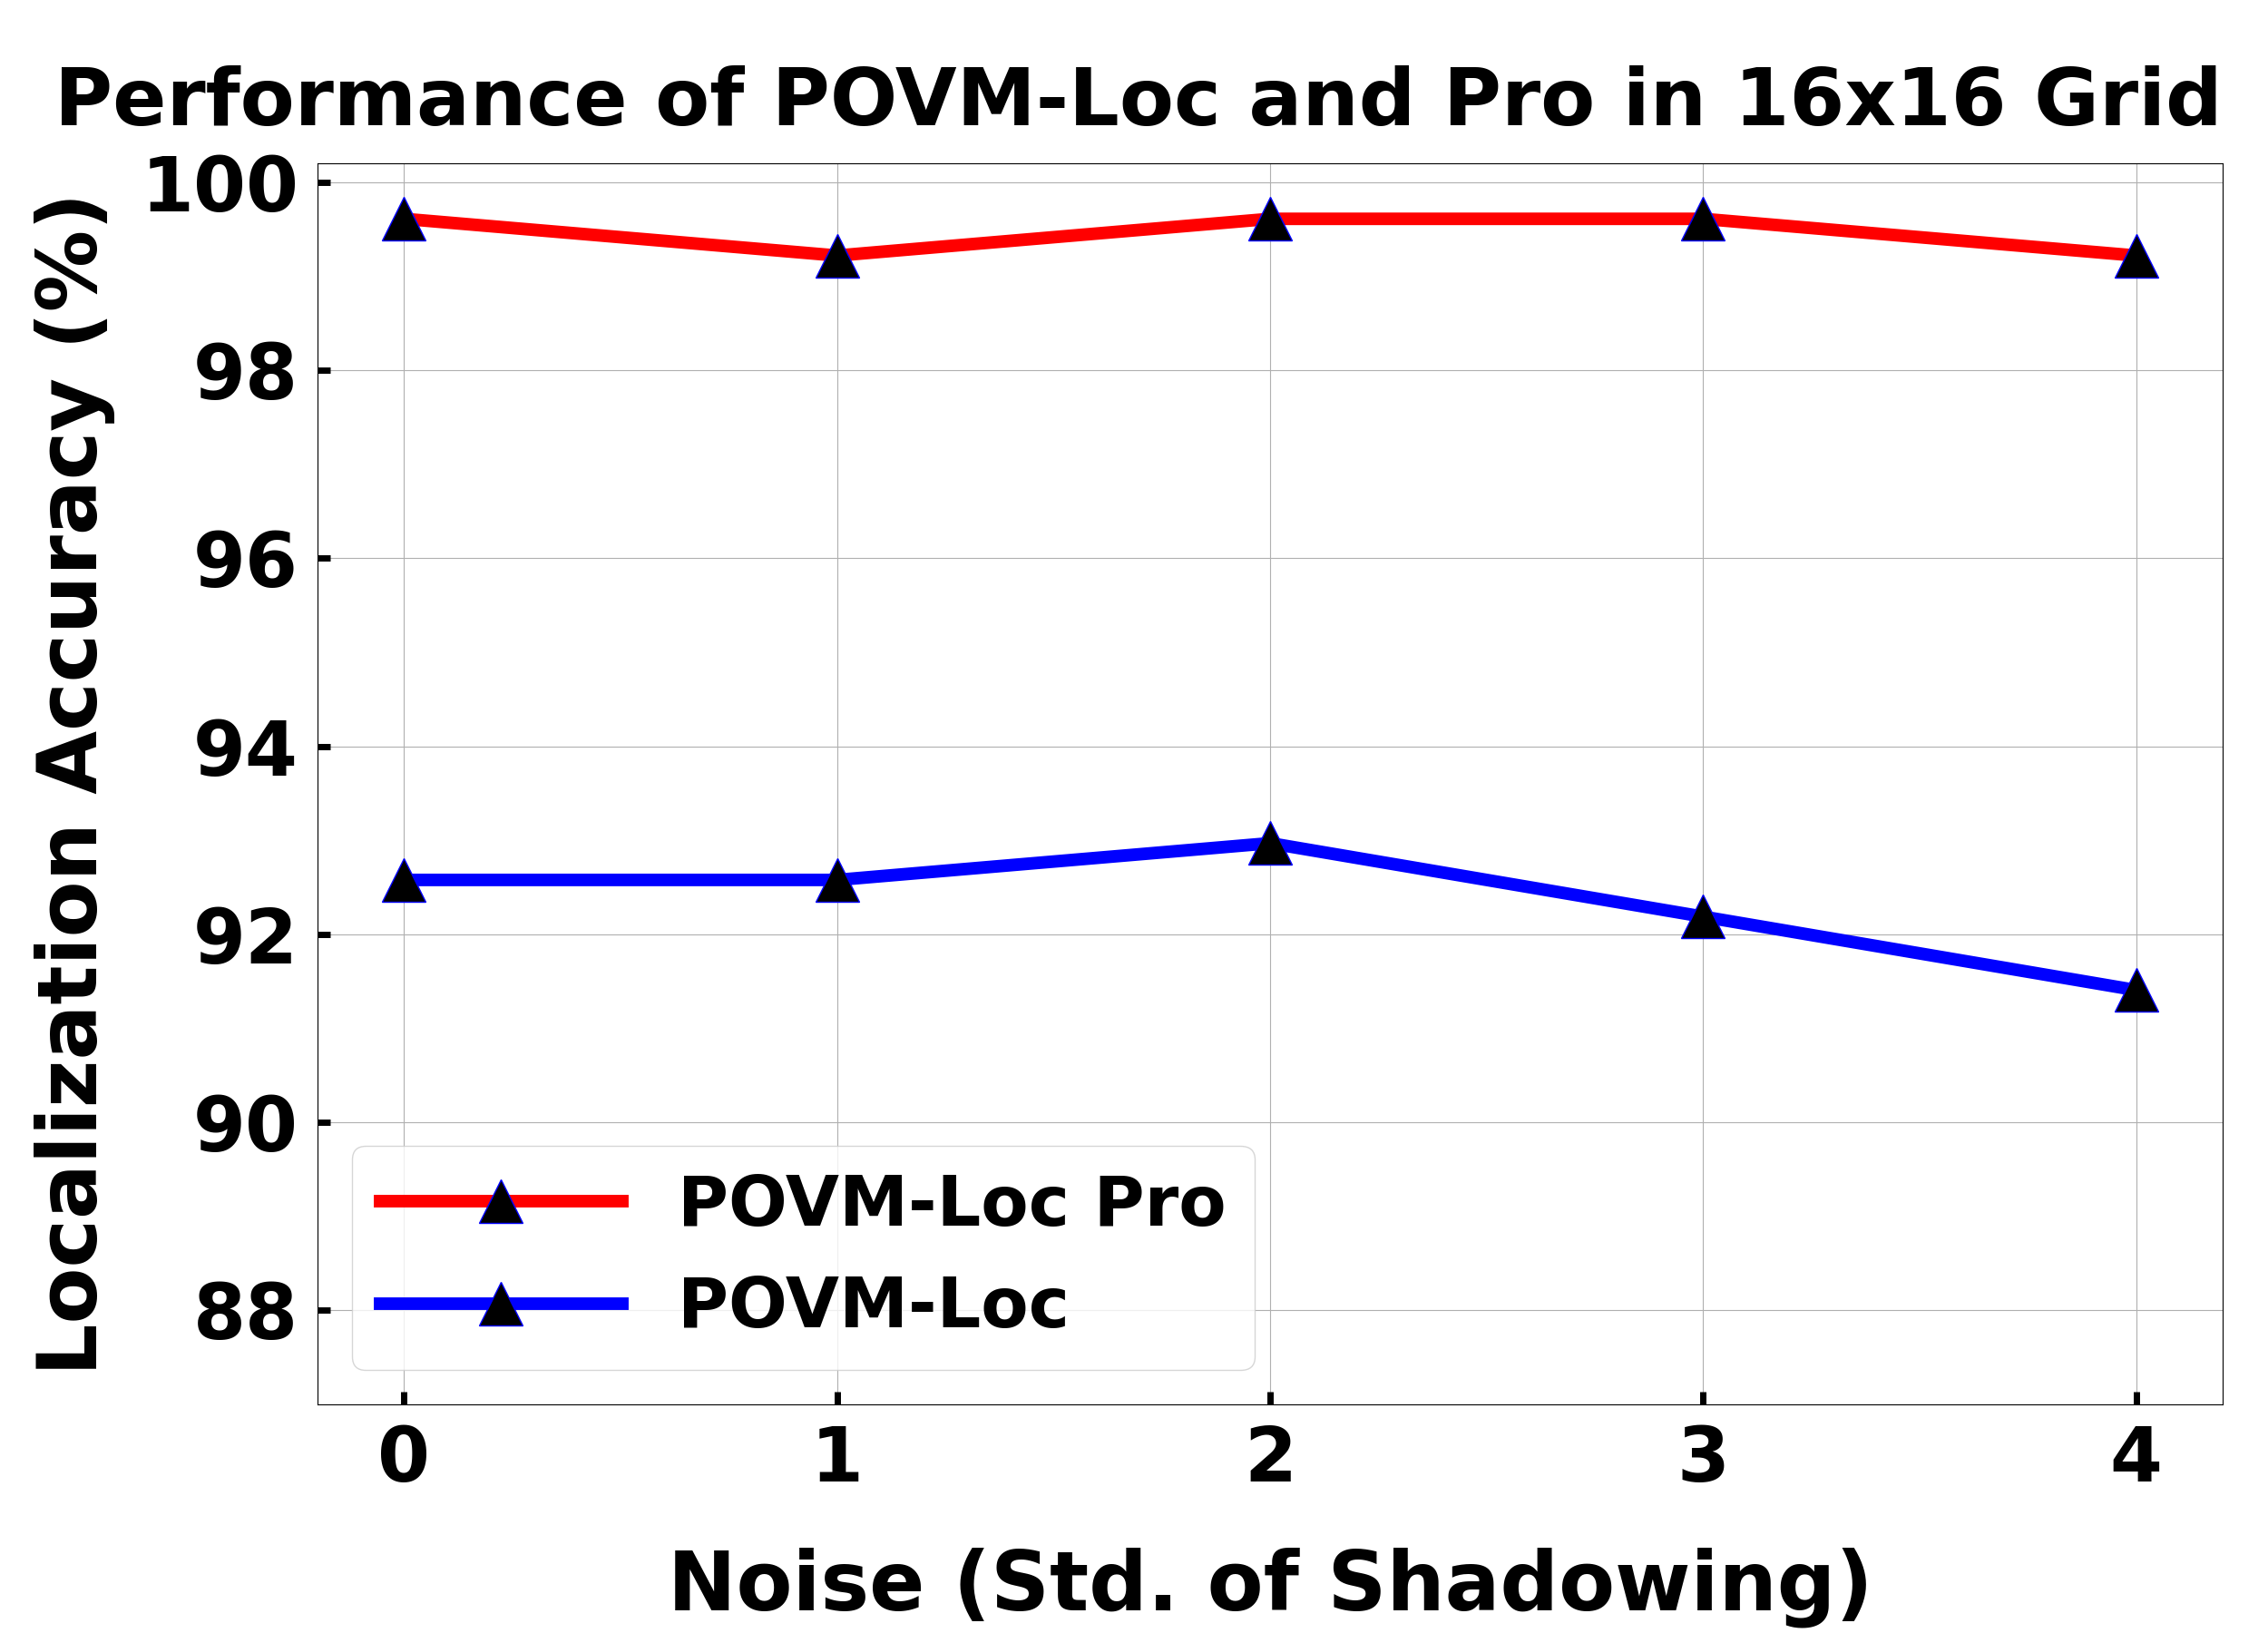
\includegraphics[width=0.75\textwidth]{chapters/icc/figures/twolevel-varynoise.png}
    % \vspace{-0.1in}
    \caption{The performance of \povm and \povmpro in $16\times 16$ grid against varying noise represented by the standard deviation in the shadowing effect (see Equation~\ref{equ:propagation}).}
    % \vspace{-0.1in}
    \label{fig:povmloc}
\end{figure}


\begin{figure}[t]
    \centering
    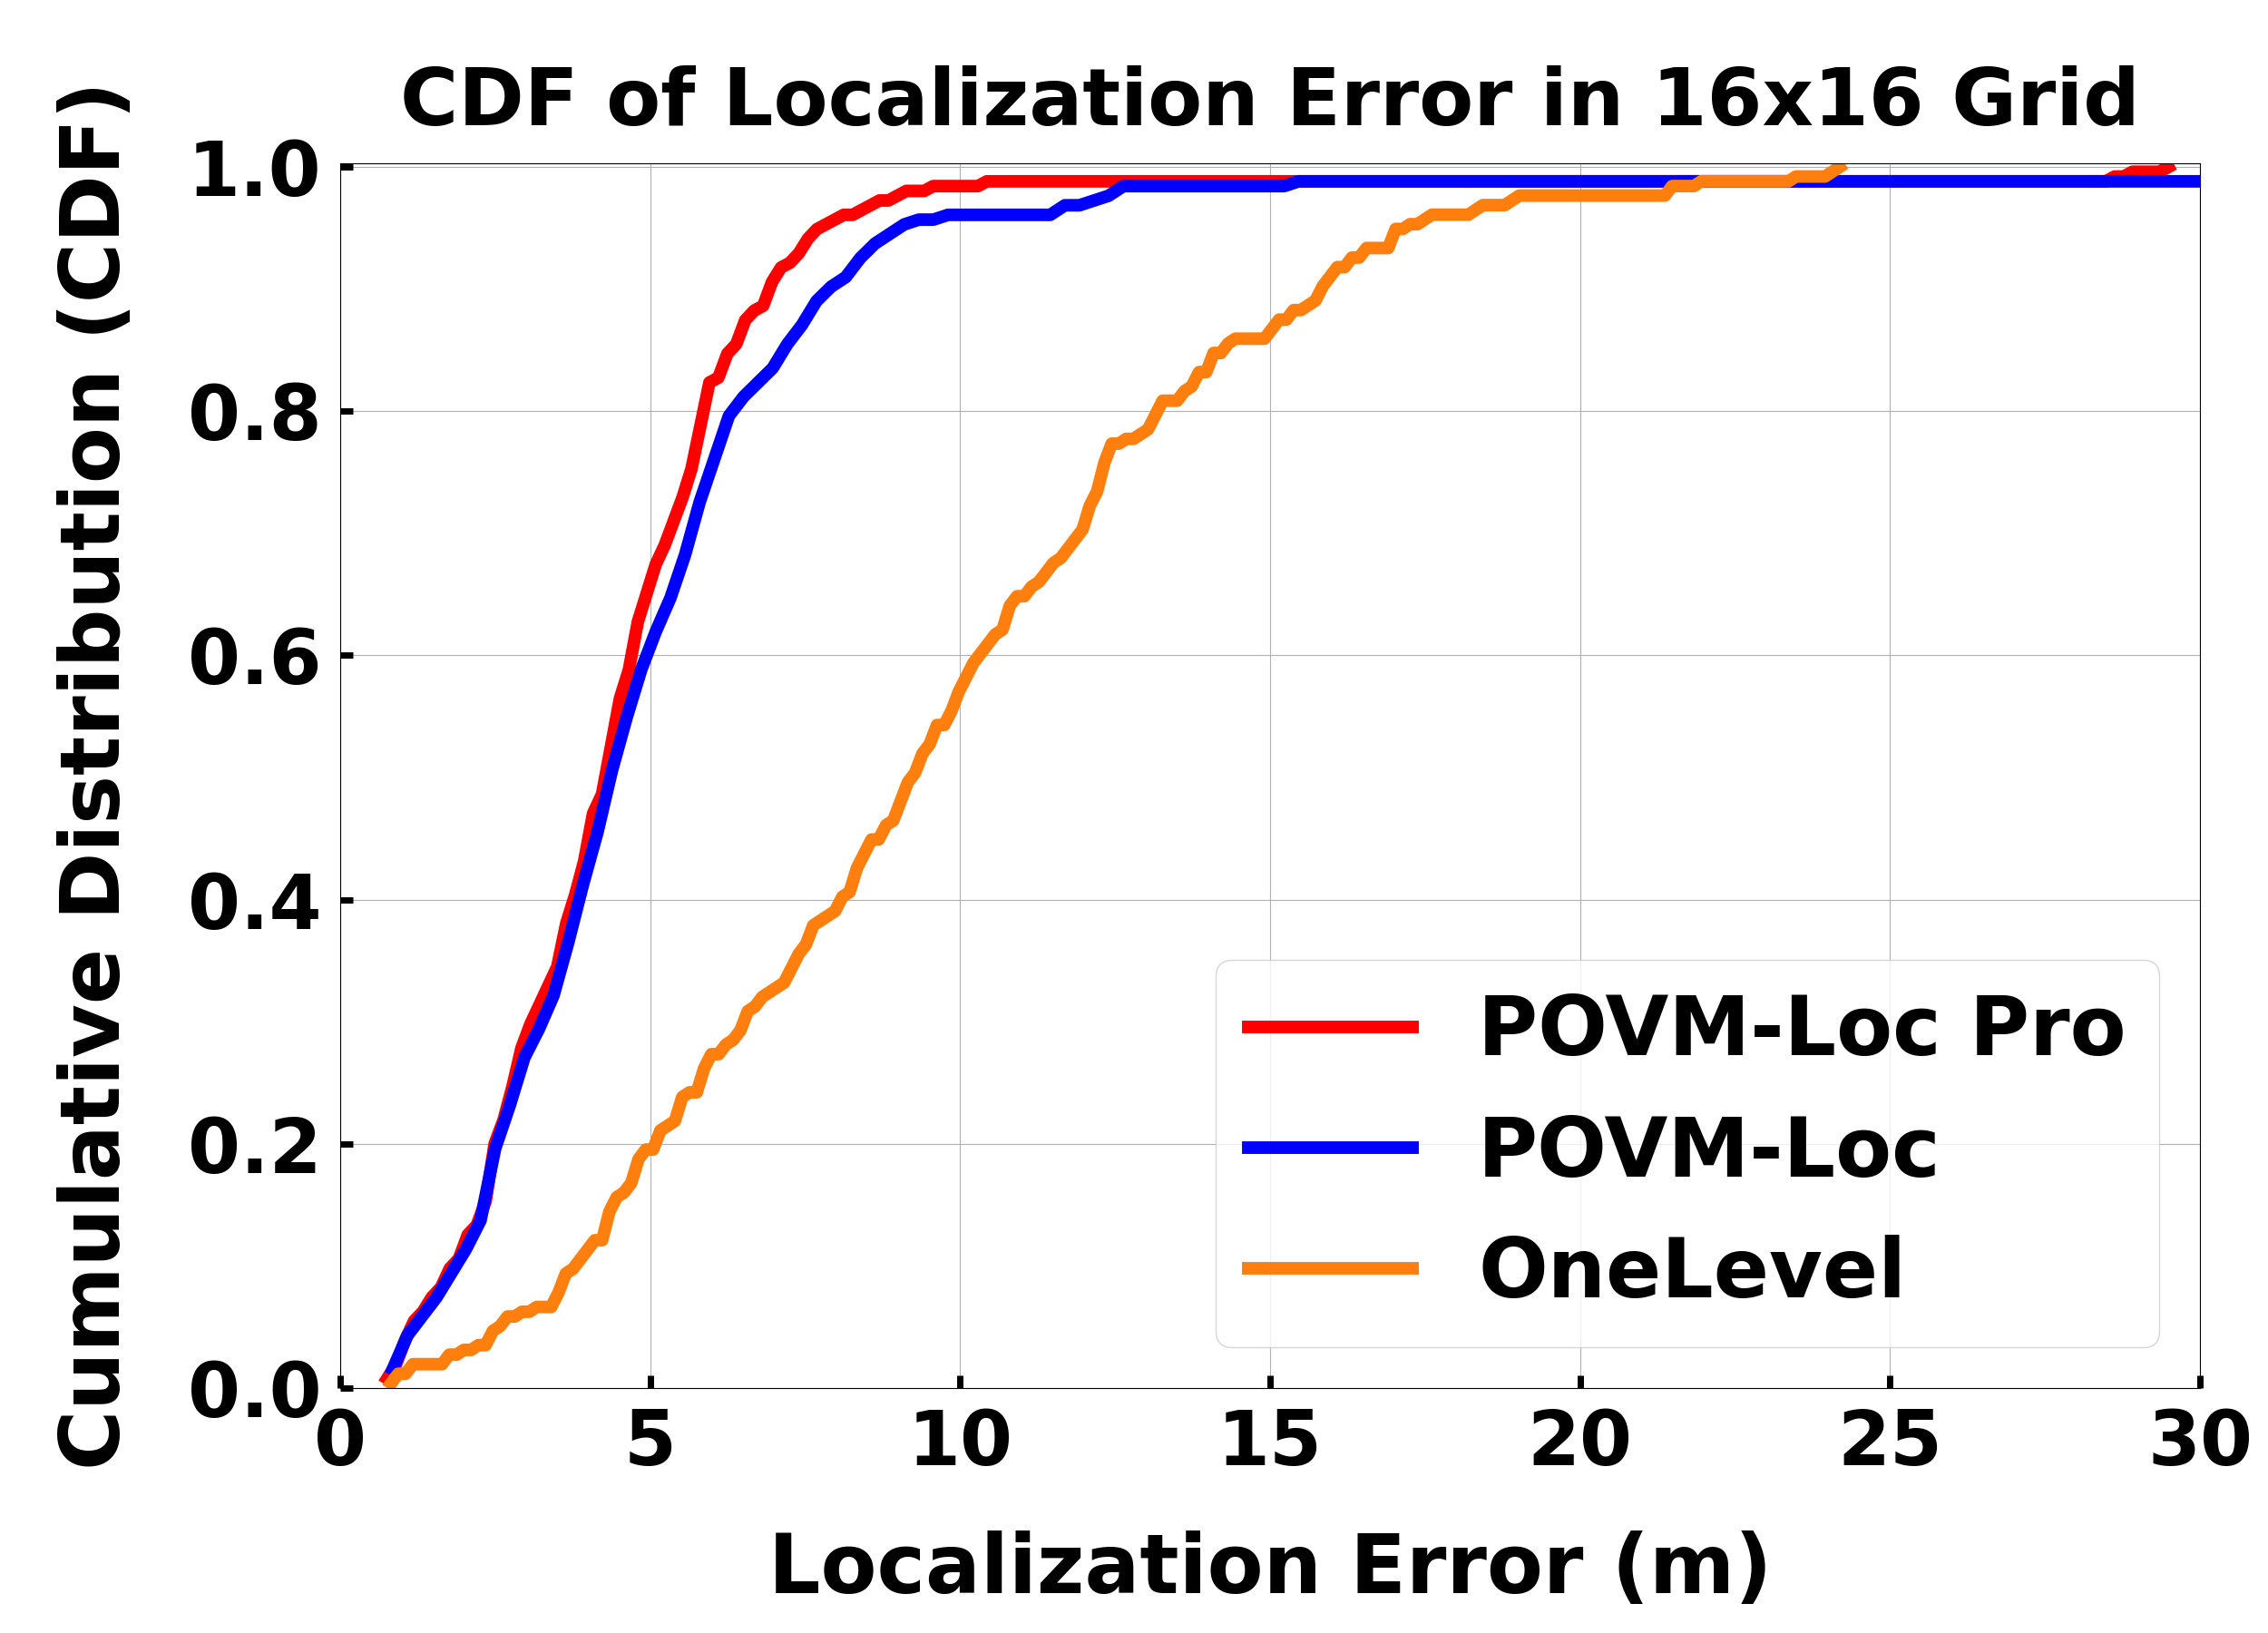
\includegraphics[width=0.75\textwidth]{chapters/icc/figures/error_cdf.png}
    % \vspace{-0.1in}
    \caption{The cumulative probability of localization of \povm, \povmpro, \povmone in a continuous and $16\times16$ grid setting.}
    % \vspace{-0.1in}
    \label{fig:errorcdf}
\end{figure}

\begin{table}[h]
\centering
\caption{Runtime (s) for \povmone using 4 and 8 quantum sensors against varying grid size}
% \vspace{-0.1in}
\begin{tabular}{||c | c | c|  c | c | c | c||} 
 \hline
  & 2x2 & 4x4 & 6x6 & 8x8 & 12x12 & 16x16\\
 \hline
 4 Sensors & 1.0 & 1.1 & 1.2 & 1.4 & 2.0 & 2.6\\ 
 \hline
 8 Sensors & 4.8 & 9.1 & 27.4 & 53.1 & 113.4 & 193.8\\ 
 \hline
\end{tabular}
% \vspace{-0.15in}
\label{tab:runtime-onelevel}
\end{table}

\begin{table}[h]
\centering
\caption{Runtime (s) for three methods in $16\times 16$ grid}
% \vspace{-0.1in}
\begin{tabular}{|| c | c | c ||} 
 \hline
 \povmone & \povm & \povmpro\\ 
 \hline
 193.8 & 10.3 & 11.3 \\ 
 \hline
\end{tabular}
% \vspace{-0.15in}
\label{tab:runtime-compare}
\end{table}

\para{The Improvement of \povm and \povmpro.}
\povm and \povmpro are evaluated in a $16\times16$ grid that is divided into $4$ rows and $4$ columns of blocks where each block's size is $4\times4$.
There are another 21 border blocks for \povmpro.
There are 8 coarse-level quantum sensors and 40 fine-level quantum sensors.
At the fine level, each block will be covered by 4 fine-level sensors.
A sensor at the border of blocks can cover either block to reduce the total sensor used.
\povm and \povmpro's improvement of localization accuracy compared with \povmone is major.
Fig.~\ref{fig:povmloc} shows the localization accuracy of \povm and \povmpro at noise equals 1 is $92.5\%$ and $99.2\%$ respectively.
At the same noise level, the localization accuracy of \povmone is only $11.7\%$ and $29.7\%$ using 4 and 8 quantum sensors respectively.
Although the total number of quantum sensors deployed for \povm and \povmpro is a lot higher than \povmone, localizing a single instance  costs only a small number of extra sensors.
\povm uses 12 sensors (8 coarse, 4 fine) and \povmpro uses a couple more.
Table~\ref{tab:runtime-compare} shows that in simulation, 
\povm and \povmpro are a lot faster than \povmone in the $16\times 16$ grid test case.
\povmpro's additional step costs 1 second more compared with \povm.
Fig.~\ref{fig:povmloc} also shows that \povm and \povmpro are robust against noise, i.e., when the noise level increases, the performance barely drops.
This robustness is due to the one thousand repetitions in Procedure~\ref{algo:sense-measure}.
For the general case of transmitter location in the continuous domain, the cumulative distribution of localization error in Fig.~\ref{fig:errorcdf} shows \povm and \povmpro also outperforms \povmone by a large margin.
While the error under $60\%$ cumulative is the same, \povmpro is better than \povm in the above $60\%$ cumulative range.

